\documentclass[a4paper]{ltxdoc}

\usepackage{url}
\usepackage{graphicx}
\graphicspath{{figures/}}
\usepackage{hyperref}
\usepackage{pdfpages}
\usepackage{geometry}
\usepackage{array,tabularx,booktabs}
\usepackage{xltabular}
\usepackage{threeparttablex}
\usepackage{capt-of}
\usepackage{makecell}

\newcommand{\baposter}{\texttt{baposter}}
\newcommand\OR{$\,\vert\,$}
\title{The \baposter{} \LaTeX{} poster class}
\author{Brian Amberg and Reinhold Kainhofer\\
Updated by Pieter van Oostrum}

\setlength{\parindent}{0pt}
\setlength{\parskip}{0.5ex}
\raggedbottom

\begin{document}
\maketitle
\begin{abstract}
\centering
This is a compact documentation of version 3.0 of the \baposter{} class.
\end{abstract}

\section{Introduction}
\baposter{} is a LaTeX template to efficently design pretty posters for
scientific conferences. Posters are composited of blocks with headings, which
can be positioned easily on the page, using absolute or relative positioning. A
number of predefined styles can be composed to generate new color schemes and
ornaments.

This document describes version 3.0 of the \baposter{} class. This version has a few new features and several bug fixes. Some bug fixes are not backwards compatible. For example, the \meta{Eye Catcher} and \meta{Logo} parameters of the \texttt{poster} environment in previous versions were (erroneously) typeset with the `\texttt{nullfont}', which made them disappear if they consisted of just text. This also generated warnings about missing characters in the \texttt{nullfont} in the log file. The text would only appear if it was embedded in for example a \cs{parbox}, in a  \texttt{tikzpicture} node, or similar.
In this version, however, the text does also appear if it is given directly as the argument.

\section{Usage}

The overall structure of a poster document is
\\[2ex]
\cs{documentclass}\oarg{class options}|{baposter}|
\\[1ex]
\meta{preamble}: additional packages, macros, definitions etc.
\\[1ex]
|\begin{document}|\\
|\begin{poster}{|\meta{poster options}|}|\\
|  { |\meta{Eye Catcher}, empty if option |eyecatcher=false }|\\
|  { |\meta{Poster Title}| }|\\
|  { |\meta{Poster Authors}| }|\\
|  { |\meta{Logo}| }|
\\[1ex]
|  |\meta{Definition of the posterboxes}
\\[1ex]
|\end{poster}|\\
|\end{document}|
\vspace{1ex}

The \texttt{poster} environment should be immediately inside
|\begin{document} / \end{document}|,

otherwise there might be blank pages.

However, you can have multiple posters in one document by including multiple \texttt{poster} environments.

\subsection{Document class options}

The following options can be given to the documentclass:

\subsubsection*{Paper size options}

\begin{tabular}{@{}>{\ttfamily}l l @{\quad}|@{\quad} >{\ttfamily}l l@{}}
  \toprule
option  & paper size       & option          & paper size          \\
  \midrule
a0paper & 841mm x 1189mm   & archA           & 9in x 12in          \\
a1paper & 594mm x 841mm    & archB           & 12in x 18in         \\
a2paper & 420mm x 594mm    & archC           & 18in x 24in         \\
a3paper & 297mm x 420mm    & archD           & 24in x 36in         \\
a4paper & 210mm x 297mm    & archE           & 36in x 48in         \\
a5paper & 148mm x 210mm    & archE1          & 30in x 42in         \\
a6paper & 105mm x 148mm    & archE2          & 26in x 38in         \\
b0paper & 1000mm x 1414mm  & archE3          & 27in x 39in         \\
b1paper & 707mm x 1000mm   & ansiapaper      & 8.5in x 11in        \\
b2paper & 500mm x 707mm    & ansibpaper      & 11in x 17in         \\
b3paper & 353mm x 500mm    & ansicpaper      & 17in x 22in         \\
b4paper & 250mm x 353mm    & ansidpaper      & 22in x 34in         \\
b5paper & 176mm x 250mm    & ansiepaper      & 34in x 44in         \\
b6paper & 125mm x 176mm    & letterpaper     & 8.5in x 11in        \\
screen  & 225mm x 180mm    & legalpaper      & 8.5in x 14in        \\
        &                  & executivepaper  & 7.25in x 10.5in     \\
\bottomrule
\end{tabular}

\subsubsection*{Other \texttt{documentclass} options}

\begin{tabularx}{\textwidth}{@{}*{2}{>{\ttfamily}l} X@{}}
\toprule
option & default & meaning \\
\midrule
portrait    & portrait &  page layout portrait \\
landscape   & - & page layout landscape \\
paperwidth  & 841mm & paper width (*) \\
paperheight & 1189mm & paper height (*) \\
fontscale   & 0.292 & scale factor.  The poster is typeset with
standard font sizes on a `\texttt{fontscale} $\times$ papersize' paper, and then scaled up
by 1/\texttt{fontscale} to the chosen paper size. This ensures good looking font sizes.
So if you need to fit more onto a poster, increase the fontscale option to get
smaller fonts. Be sure not to choose too small fonts, or your poster will be awful. \\
margin      &   1.5cm & base margin around the text \\
movebody    & 0cm & amount to move the text to the right (left if negative) \\
debug       & false & \texttt{true\OR false}; if \texttt{true} output debug info to log file \\
table       & - & passsed to the \texttt{xcolor} package \\
showframe   & - & passed to the \texttt{geometry} package, show a frame around the page for debugging. \\
\bottomrule
\multicolumn{3}{l}{(*) Do not use together with a page size option.}
\end{tabularx}

\section{The \texttt{poster} environment}

The environment for the whole poster is \texttt{poster}. 
\\[2ex]
|\begin{poster}|\marg{poster options}\\
|   |\marg{Eye Catcher} \\
|   |\marg{Poster Title} \\
|   |\marg{Poster Authors}  \\
|   |\marg{Logo}
\\[1ex]
|  |\meta{Posterboxes}
\\[1ex]
|\end{poster}|\\[1ex]

Please note that the \meta{poster options} are given in curly braces \texttt{\{ \}}, not in square brackets \texttt{[ ]}.

\meta{Eye Catcher} and \meta{Logo} are often images, but they can also be just text.
%\meta{Eye Catcher} is subject to the \texttt{eyecatcher} option:

The layout of the poster header depends on the \texttt{eyecatcher} option.
If  \texttt{eyecatcher=true}, the  \meta{Title} and \meta{Authors} are typeset centered between the  \meta{Eye Catcher} and the \meta{Logo} (figure~\ref{with-eye-catcher}), even when the \meta{Eye Catcher} parameter is left empty (figure~\ref{with-empty-eye-catcher}).

On the other hand, if \texttt{eyecatcher=false}, the \meta{Eye Catcher} is omitted, even when given as a parameter.
In this case the \meta{Title} and \meta{Authors} are typeset left aligned (figure~\ref{without-eye-catcher}).

\begin{figure}[hbtp]
  \centering
  \setlength{\fboxsep}{0pt}
  \fbox{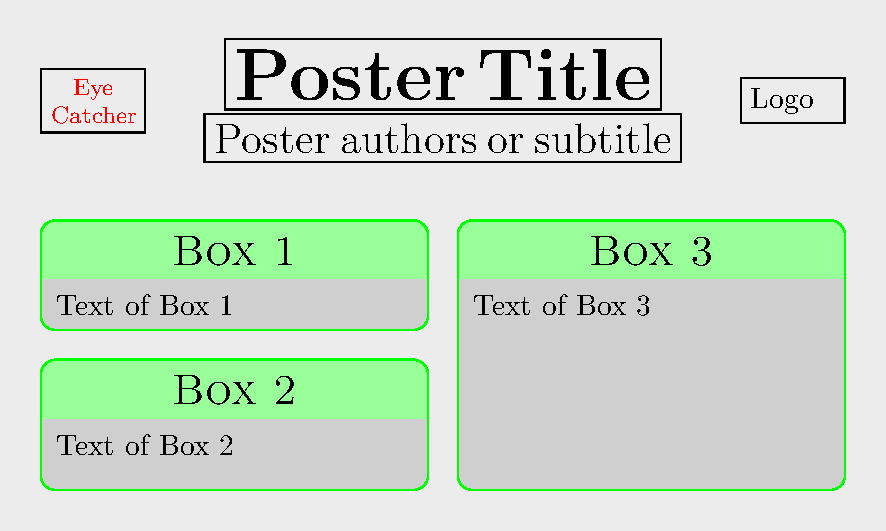
\includegraphics[width=0.9\textwidth]{docs-structure1}}
  
  \caption{Poster layout with \texttt{eyecatcher=true} and non-empty \meta{Eye Catcher}}
  \label{with-eye-catcher}
\end{figure}

\begin{figure}[hbtp]
  \centering
  \setlength{\fboxsep}{0pt}
  \fbox{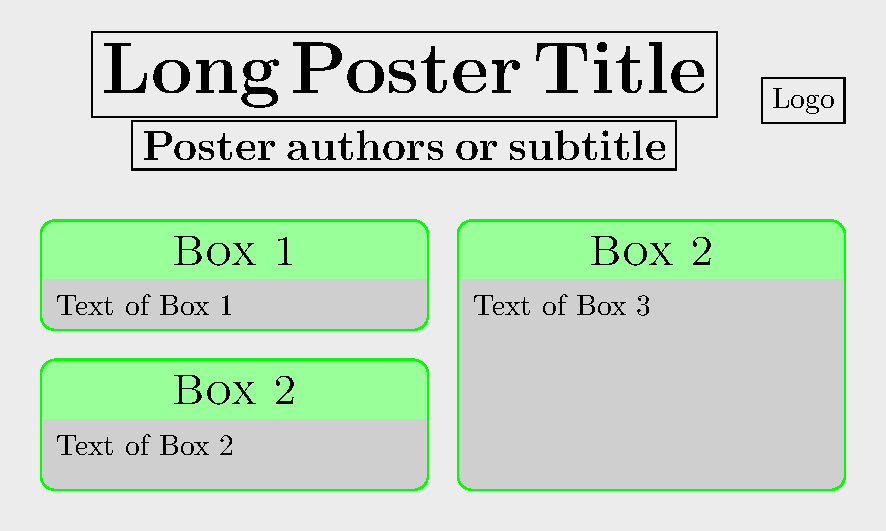
\includegraphics[width=0.9\textwidth]{docs-structure3}}
  
  \caption{Poster layout with \texttt{eyecatcher=true} and empty \meta{Eye Catcher}}
  \label{with-empty-eye-catcher}
\end{figure}

\begin{figure}[hbtp]
  \centering
  \setlength{\fboxsep}{0pt}
  \fbox{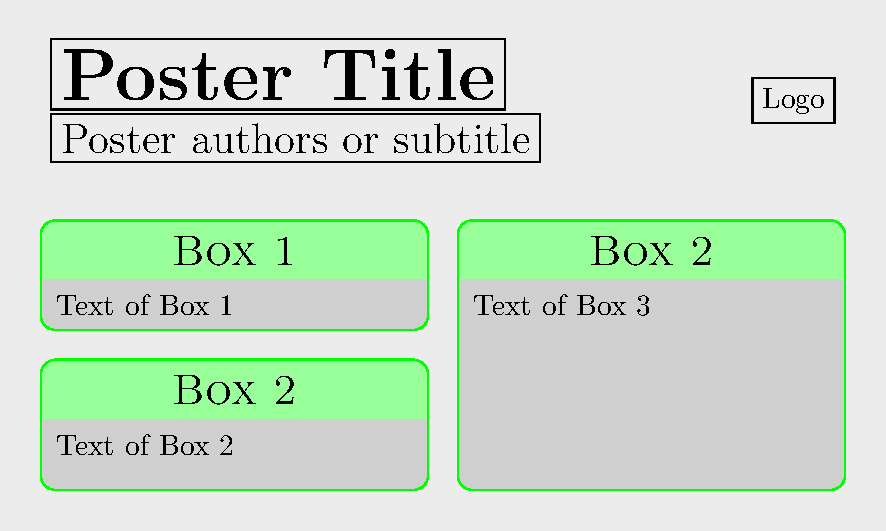
\includegraphics[width=0.9\textwidth]{docs-structure2}}
  
  \caption{Poster layout with \texttt{eyecatcher=false} (no \meta{Eye Catcher})}
  \label{without-eye-catcher}
\end{figure}


\subsection{\texttt{Poster} environment options}

The available options are (see table~\ref{options-poster}):\\
\textbf{Note:} All colors from the \texttt{xcolor} package can be used for the \meta{color} options.

\begin{center}
\begin{ThreePartTable}
  \begin{TableNotes}
    \item[1] Actually, \texttt{baposter@silver}, defined as \texttt{\{cmyk\}\{0,0,0,0.7\}}.
  \end{TableNotes}
\begin{xltabular}{\textwidth}{@{}*3{>{\ttfamily}l} X@{}}
\caption{Options for \texttt{poster} environment}\label{options-poster}\\
  \toprule
option       & \normalfont value           & default & meaning \\
  \midrule
\endfirsthead
  \toprule
option       & \normalfont value           & default & meaning \\
  \midrule
\endhead
  \bottomrule
\endfoot
\bottomrule
\insertTableNotes
\endlastfoot
%
eyecatcher   & true\OR false & true & Should an eye catcher be shown on the
 left of the title page. The eyecatcher itself is defined in the second
 argument of the poster environment \\
grid         & true\OR false & false & Display a grid, which can be useful during the layout phase \\
columns      & \meta{int}     & 3\OR 4 & Number of columns, default 3 in portrait and 4 in landscape format; maximum number is 6 \\
colspacing   & \meta{length}  & 1em & Horizontal distance between the columns of the poster \\
headerheight & \meta{length}  & 0.1\cs{textheight} & Height of the main poster header as a length (not of the headers of the text boxes) \\
titlefont    & \meta{font}    &
             \multicolumn{2}{l}{\cs{bfseries}\cs{Huge}\cs{baselineskip}\texttt{=2.2ex}} \\
  & & &            Font commands applied to the poster title \\
authorfont   & \meta{font} &
             \multicolumn{2}{l}{\cs{Large}\cs{baselineskip}\texttt{=2.2ex}} \\
  & & &             Font commands applied to the Authors in the title \\
background   & See Table~\ref{options-bg}       & plain &  Type of poster background.\\
bgColorOne   & \meta{color} & `silver'\tnote{1} & First background color. For a \texttt{plain}, this color will be used. For a shaded background, this is the first color for the gradient \\
bgColorTwo   & \meta{color} & green & Second background color. This color will only be used for shaded backgrounds as the end color of the gradient \\
\end{xltabular}
\end{ThreePartTable}

\begin{ThreePartTable}
  \begin{TableNotes}
    \item[*] These values are case insensitive, so instead of \texttt{shadelr} you can also say \texttt{shadeLR} or \texttt{ShadeLR} if you want
    \item[1] Only for \texttt{posterbox} \texttt{headershade} option
    \item[2] Only for \texttt{poster} \texttt{background} option
  \end{TableNotes}
\begin{xltabular}{\textwidth}{@{}*3{>{\ttfamily}l} X@{}}
\caption{Options for \texttt{background/shade}}\label{options-bg}\\
\toprule
value\tnote{*} & meaning \\
\midrule
\endfirsthead
\toprule
option       & \normalfont value           & default & meaning \\
\midrule
\endhead
\bottomrule
\endfoot
\bottomrule
\insertTableNotes
\endlastfoot
 plain     & Plain background in one color (\texttt{bgColorOne}) \\
 shadelr   & Horizontal background gradient (from \texttt{bgColorOne} to \texttt{bgColorTwo}) \\
 shadetb   & Vertical background gradient (from \texttt{bgColorOne} to \texttt{bgColorTwo}) \\
 shadetbinverse\tnote{1} & Variant of \texttt{shadetb}, which is slightly rotated \\
 user\tnote{2}      & Use the command \cs{background} to define your own background. \\
 none      & No background at all. \\
\end{xltabular}
\end{ThreePartTable}
\end{center}

 
\begin{figure}[htb]
\centering
    \setlength{\fboxsep}{0pt}

    \fbox{
\includegraphics[width=0.21\textwidth,page=1]{docs-background}}
    \fbox{
\includegraphics[width=0.21\textwidth,page=2]{docs-background}}
    \fbox{
\includegraphics[width=0.21\textwidth,page=3]{docs-background}}
    \fbox{
\includegraphics[width=0.21\textwidth,page=4]{docs-background}}
    \caption{Poster backgrounds}
    \label{poster-backgrounds}
\end{figure}

\section{The \texttt{posterbox} environment}

The environment for a box in the poster is \texttt{posterbox}. 
\\*[2ex]
|\begin{posterbox}|\oarg{posterbox options}\marg{Posterbox Title}
\\*[1ex]
|  |\meta{Posterbox contents}
\\*[1ex]
|\end{posterbox}|\\[1ex]

Each box has a name and can be placed absolutely or relatively.
The only inconvenience is that you can only specify a relative position 
towards an already declared box. So if you have a box attached to the 
bottom, one to the top and a third one which should be inbetween, you 
have to specify the top and bottom boxes before you specify the middle 
box.

\subsection{\texttt{Posterbox} environment options}

\textbf{Note:} The \texttt{posterbox} options can also be given in the options parameter of the \texttt{poster} environment. They will then be applied to all the \texttt{posterbox}es, unless specifically overridden there. This is especially useful for \texttt{posterbox} options that are the same for all boxes.

\begin{ThreePartTable}
  \begin{TableNotes}
    \item[*] The first value is used if the option is not given; the second one (in parentheses) is used when the option is given without a value.
  \end{TableNotes}
\begin{xltabular}{\textwidth}{@{}*3{>{\ttfamily}l} @{ }X@{}}
\caption{Options for \texttt{posterbox} environment}\label{options-posterbox}\\
\toprule
option       & \normalfont value           & default & meaning \\
\midrule
\endfirsthead
\toprule
option       & \normalfont value           & default & meaning \\
\midrule
\endhead
\bottomrule
\endfoot
\bottomrule
\insertTableNotes
\endlastfoot
%
\multicolumn{3}{@{}l}{\textit{Position:}} \\*
%\midrule
name          & \meta{string}   & noname & Name of the box, used to refer to position other boxes \\
column        & \meta{int}      & 0      & Column number where to position the box \\
row           & \meta{number}      & 0      & Row number where to position the box; this is the fraction of the poster height. With the default poster header height 0.1 will be the top row for boxes. \\
span          & \meta{int}      & 1      & How many columns the box should occupy \\
aligned       & \meta{name}     & notset & Name of box to align the top of this box with \\
bottomaligned & \meta{name}     & notset & Name of box to align the bottom of this box with \\
below         & \meta{name}     & notset & Name of box where this box is positioned below \\
above         & \meta{name}     & notset & Name of box where this box is positioned above \\
height        & auto\OR         & auto   & Box height: if \texttt{auto}, height is determined by contents of the box;\\*
              & bottom\OR       &        & if \texttt{bottom}, it stretches out until the bottom of the poster;\\*
              & \meta{number}   &        & if a number, it is the fraction of the column height of the poster \\
%
%\midrule
\multicolumn{3}{@{}l}{\textit{Box design: border:}} \\*
%\midrule
linewidth     & \meta{length}   & 2pt    &  Width of the lines to draw the box \\
borderColor   & \meta{color}    & yellow & Color used for the borders of the poster boxes \\
cornerradius  & \meta{length}   & 1em    & Radius of corners for rounded corners \\
%
%\midrule
\multicolumn{3}{@{}l}{\textit{Box design: header:}} \\*
%\midrule
headerfont    & \meta{font}    & \multicolumn{2}{l}{\cs{scshape}\cs{Large}} \\*
  & & & Commands inserted before a text box header is typeset \\
headerFontColor & \meta{color} & black   & Color that the header is typeset in \\
headerColorOne   & \meta{color} & red    & First \texttt{headershade} color. For a \texttt{plain} header, this color will be used. For a shaded header, this is the first color for the gradient \\
headerColorTwo   & \meta{color} & brown  & Second header color. This color will only be used for shaded headers as the end color of the gradient \\
headershape  & See figure~\ref{fig:headershape} & \makecell[tl]{rectangle\tnote{*}\\(roundedright)} & The type of ornament of the text box headers \\
headershade   & See table~\ref{options-bg} & shadelr & Which shading should be applied to the text box headers. See also figure~\ref{fig:headershade} \\
headerborder  & See figure~\ref{fig:headerborder} & \makecell[tl]{none\tnote{*}\\(open)} & What border should we draw on the text box header \\
boxheaderheight & \meta{length} & 2em    & Height of the header \\
%
%\midrule
\multicolumn{3}{@{}l}{\textit{Box design: text:}} \\*
%\midrule
textfont   & \meta{font} & \textit{none} & Commands inserted before a text box is typeset \\*
  & & & Font commands applied to the Authors in the title \\
boxshade     &  See table~\ref{options-bg} & none & Which kind of shading is applied to the text boxes \\
boxColorOne   & \meta{color} & magenta  & First \texttt{boxshade} color. For a \texttt{plain} box, this color will be used. For a shaded box, this is the first color for the gradient \\
boxColorTwo   & \meta{color} & cyan  & Second box color. This color will only be used for shaded boxes as the end color of the gradient \\
textborder   & See figure~\ref{fig:textborder} & \makecell[tl]{faded\tnote{*}\\(rectangle)} & Which kind of border should the lower part of the text boxes have \\
boxpadding   & \meta{length} & 0.5em     & Amount of padding around the box contents \\
boxopacity   & \makecell[tl]{\meta{number}\\(0.0-1.0)} & 1.0 & Opacity of the box background (header and text) \\
\end{xltabular}
\end{ThreePartTable}

\begin{figure}[htbp]
  \centering
  \caption{Header shade types}
  \label{fig:headershade}
  
\includegraphics[width=0.9\textwidth]{docs-headershade}
\end{figure}

\begin{figure}[htbp]
  \centering
  \caption{Headerborder types}
  \label{fig:headerborder}
  
\includegraphics[width=0.9\textwidth]{docs-headerborder}
\end{figure}

\begin{figure}[htbp]
  \centering
  \caption{Header shape types}
  \label{fig:headershape}
  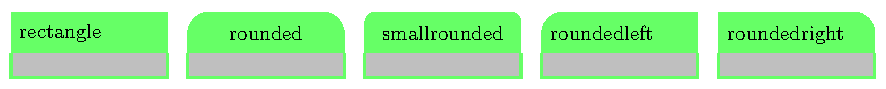
\includegraphics[width=0.9\textwidth]{docs-headershape}
\end{figure}

\begin{figure}[htbp]
  \centering
  \caption{Textborder types}
  \label{fig:textborder}
  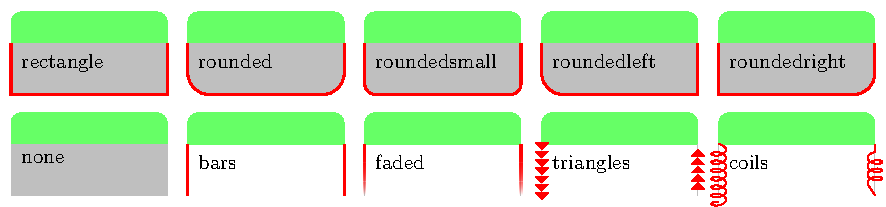
\includegraphics[width=0.9\textwidth]{docs-boxshape}
\end{figure}

\subsection{\texttt{Posterbox} contents}

The \baposter{} documentclass is based on the standard \LaTeX{} documentclass \texttt{article}. As such you can use most of the commands and environments that this class defines. You can also load other packages, as long as they don't take over the \LaTeX{} page. 

Some examples of compatible packages are: \texttt{amsmath}, \texttt{mathtools}, \texttt{multicol},
\texttt{tikz} (\texttt{tikz} is heavily used in \baposter{}, so you don't even have to include it yourself), \texttt{xcolor}, \texttt{graphics/graphicx}, \texttt{tabularray}, \texttt{tabularx}, but there are many more.
Experience must show whether a package really is compatible.

If you want to use multi-column text inside a box, this can be done with the \texttt{multicol} package, and the \texttt{multicols} environment. However this usually makes only sense when you have wider boxes. The \texttt{examples} directory in the distribution has a couple of examples where this is used. See also figure~\ref{fig:example-boxes}.

What you cannot do in a posterbox is to use the \texttt{figure} and \texttt{table} environments or similar other floating environments. These cannot be used inside a box, and it wouldn't make sense to float them anyway.

What you can do is to include a \texttt{tabular} or similar environment directly in the text. In the same way you can include a figure with the \cs{includegraphics} command, or construct it with \texttt{tikz} or other similar packages. However, this doesn't give you captions.

To use captions you can use the package \texttt{caption} or \texttt{capt-of}, which offer a command \cs{captionof}. If this is the only command you need, then \texttt{capt-of} is the better choice as it only defines this command, and therefore is very small.

A good way to emulate a \texttt{table} environment is for example:

\begin{minipage}{\textwidth}
\begin{verbatim}
\begin{center}
  \begin{tabular}{llr}
    \hline
    Experiment & Year & Result \\
    \hline
    1          & 2020 & 2.35 \\
    2          & 2021 & 7.47 \\
    3          & 2022 & 1.98 \\
    \hline
  \end{tabular}
  \captionof{table}{Experimental results}
\end{center}
\end{verbatim}
\end{minipage}
\begin{figure}[htbp]
  \centering
  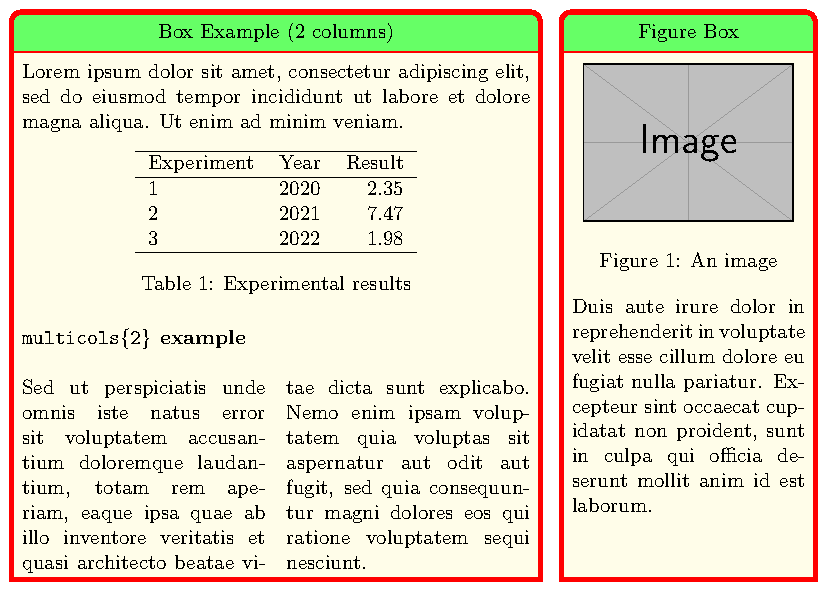
\includegraphics{docs-table-example}
  \caption{Example boxes with a table, a figure and
    \texttt{multicols\{2\}}}
  \label{fig:example-boxes}
\end{figure}

The \texttt{center} environment not only centers its contents horizontally (which is often what you want), but it also gives a little vertical space before and after the table to separate it from the surrounding text. Of course you can use other means to get your desired layout. And the same principle applies to figures:

\begin{minipage}{\textwidth}
\begin{verbatim}
  \begin{center}
    \includegraphics[width=0.9\linewidth]{example-image}
    \captionof{figure}{An image}
  \end{center}
\end{verbatim}
\end{minipage}

\section{Authors and Licence}
The original author is Brian Amberg, and the class and documentation has been
greatly improved by Reinhold Kainhofer. They have written the bulk of the class file.

Improvements to the code were made by Mathias Loesch, Alan Munn, and Pieter van Oostrum.

The current version of this documentation was made by Pieter van Oostrum. It was largely rewritten, but used elements from the original documentation.
It can be found at:
\begin{center}
  \url{https://github.com/pietvo/baposter}
\end{center}
The class is distributed under the GPL.

The original version and documentation can be found at:
\begin{center}
\url{http://www.brian-amberg.de/uni/poster/}
\end{center}

\end{document}

